% Drawing 69/04-4 -- folder 69, batch 04, archive page 77 (PDF page 78).
% Transcription: en regard des listes : un prisme triangulaire, un prisme double (deux prismes empilés), un « pseudocube » en perspective, et un hexagone traversé de trois diagonales. Au milieu de la page : un dodécaèdre gauche en perspective, ses sommets marqués $\xi_{13}$, $\xi_{45}$, $\xi_{14}$, $\xi_{23}$, $\xi_{51}$, $\xi_{24}$, $\xi_{34}$, $\xi_{12}$, $\xi_{53}$ ; plus loin un pentagone numéroté $1,\ldots,5$ avec la suite « $1\,2\,3\,4\,5$ », un pentagramme dans un carré, une petite figure fermée et un hexagone.
% Kind: page of polyhedra sketches. Method 2 (schematic redraw from the facsimile). Status: partial.
% Notes: Upper half of the page and its middle, each sketch at its place, vertices placed once and every stroke drawn between them: by the list, a small prism seen end-on (a triangle on a square, one edge inked heavier) and the double prism (two stacked boxes under a top face); the 'pseudocube' in perspective (seven vertices, the left edge thick); in the right margin a hexagon crossed by its three long diagonals (broken in the middle on the page, drawn whole); in the middle the skew dodecahedron, its outer pentagon, the inner vertices and the heavy central strokes, with a heavy quadrilateral corner to its upper left, and its labels xi_13, xi_53, xi_12, xi_14, xi_45, xi_23, xi_51 where they stand; the pentagon with '1 2 3 4 5' beside it; the pentagram figure under it; a small closed figure and a hexagon. Not drawn: the lists and computations (text). Still differs from the facsimile: the dodecahedron and the pentagram are overdrawn on the page, and only their main strokes are given (which strokes join which vertices is a reading); the small closed figure and the bottom hexagon (cut by the fold) are approximate; the further labels of the dodecahedron (xi_13 ... xi_45 in the transcription's list) that are overwritten are left out. Redrawn 2026-11-09 (issue 128): vertices placed once and every edge drawn between them, labels at \small, strike-outs not drawn; to check again.
% Coordinates: 1 unit = 1 mm = 1/100 of the crop width (bbox in page fractions: [0.05, 0.05, 0.95, 0.55]).
% Redrawn by Claude (claude-opus-5-5), issue #73, 2026-11-09; not checked by a human; not compiled (no TeX in the session).
% Rights: reproduces part of the work -- behind RENDER_TRANSCRIPTS, never published by itself.
\documentclass[tikz,border=3pt]{standalone}
\usepackage{amsmath,amssymb}
\usetikzlibrary{patterns,arrows.meta}
\tikzset{pencil/.style={black!45}, struck/.style={black!35}, mark/.style={circle,draw,inner sep=1.3pt}, pt/.style={circle,fill,inner sep=0.9pt}, opt/.style={circle,draw,fill=white,inner sep=1.1pt}}
\begin{document}
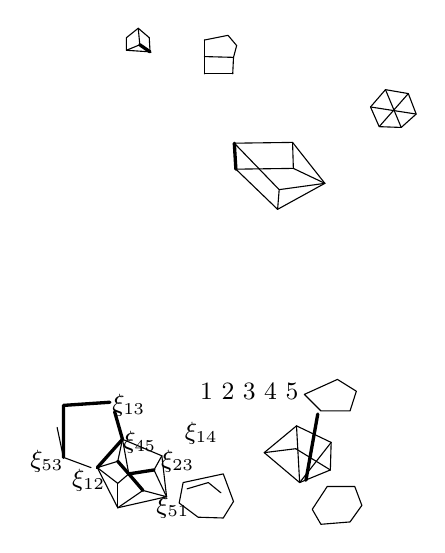
\begin{tikzpicture}[x=1mm,y=1mm,line cap=round,line join=round,font=\scriptsize]
\draw (49.2,-6.1) -- (50.7,-4.9) -- (52.1,-6.1);
\draw (49.2,-6.1) -- (49.2,-7.7) -- (52.2,-7.9) -- (52.1,-6.1);
\draw (50.7,-4.9) -- (50.9,-7);
\draw (50.9,-7) -- (49.2,-7.7);
\draw[very thick] (50.9,-7) -- (52.2,-7.9);
\draw (59.1,-6.4) -- (62.1,-5.8) -- (63.2,-7.1);
\draw (59.1,-6.4) -- (59.1,-8.5) -- (59.1,-10.7);
\draw (63.2,-7.1) -- (62.8,-8.6) -- (62.7,-10.7);
\draw (59.1,-10.7) -- (62.7,-10.7);
\draw (59.1,-8.5) -- (62.8,-8.6);
\draw (62.9,-19.5) -- (70.3,-19.4);
\draw[very thick] (62.9,-19.5) -- (63.1,-22.8);
\draw (70.3,-19.4) -- (70.4,-22.7);
\draw (70.3,-19.4) -- (74.4,-24.6);
\draw (63.1,-22.8) -- (70.4,-22.7);
\draw (63.1,-22.8) -- (68.4,-27.9);
\draw (62.9,-19.5) -- (68.6,-25.4);
\draw (68.6,-25.4) -- (68.4,-27.9);
\draw (68.4,-27.9) -- (74.4,-24.6);
\draw (70.4,-22.7) -- (74.4,-24.6);
\draw (68.6,-25.4) -- (74.4,-24.6);
\draw (82.1,-12.7) -- (85,-13.2) -- (86,-15.8) -- (84.1,-17.5) -- (81.3,-17.4) -- (80.2,-14.9) -- cycle;
\draw (82.1,-12.7) -- (84.1,-17.5);
\draw (85,-13.2) -- (81.3,-17.4);
\draw (86,-15.8) -- (80.2,-14.9);
\draw[very thick] (45.5,-60.7) -- (48.7,-57.1);
\draw (48.7,-57.1) -- (53.7,-59.2);
\draw (53.7,-59.2) -- (54.3,-64.4);
\draw (54.3,-64.4) -- (48.1,-65.8);
\draw (48.1,-65.8) -- (45.5,-60.7);
\draw (45.5,-60.7) -- (48.1,-59.9);
\draw (48.7,-57.1) -- (48.1,-59.9);
\draw[very thick] (48.1,-59.9) -- (49.5,-61.5);
\draw[very thick] (49.5,-61.5) -- (52.7,-61);
\draw[very thick] (49.5,-61.5) -- (51.3,-63.6);
\draw (49.5,-61.5) -- (48.1,-62.7);
\draw (48.7,-57.1) -- (49.5,-61.5);
\draw (52.7,-61) -- (53.7,-59.2);
\draw (52.7,-61) -- (54.3,-64.4);
\draw (51.3,-63.6) -- (48.1,-65.8);
\draw (51.3,-63.6) -- (54.3,-64.4);
\draw (45.5,-60.7) -- (48.1,-62.7);
\draw (48.1,-62.7) -- (48.1,-65.8);
\draw[very thick] (47.7,-53.6) -- (48.7,-57.1);
\draw[very thick] (47.1,-52.4) -- (41.2,-52.8) -- (41.2,-59.4);
\draw (41.2,-59.4) -- (44.7,-60.7);
\draw (40.4,-55.6) -- (41.2,-59.4);
\node[inner sep=1pt] at (49.5,-52.8) {\small $\xi_{13}$};
\node[inner sep=1pt] at (39.1,-59.9) {\small $\xi_{53}$};
\node[inner sep=1pt] at (44.4,-62.3) {\small $\xi_{12}$};
\node[inner sep=1pt] at (58.7,-56.4) {\small $\xi_{14}$};
\node[inner sep=1pt] at (50.9,-57.5) {\small $\xi_{45}$};
\node[inner sep=1pt] at (55.7,-59.9) {\small $\xi_{23}$};
\node[inner sep=1pt] at (55.1,-65.8) {\small $\xi_{51}$};
\draw (56.4,-62.6) -- (61.5,-61.5) -- (62.8,-65) -- (61.5,-67.1) -- (58.3,-67) -- (55.9,-65.2) -- cycle;
\draw (56.9,-63.4) -- (59.6,-62.6) -- (61.2,-63.9);
\draw (71.8,-51.4) -- (76,-49.5) -- (78.4,-51) -- (77.6,-53.5) -- (73.9,-53.5) -- cycle;
\node[inner sep=1pt] at (64.8,-51) {\small $1\ 2\ 3\ 4\ 5$};
\draw (66.7,-58.8) -- (70.8,-55.4);
\draw (66.7,-58.8) -- (71.2,-62.6);
\draw (66.7,-58.8) -- (70.7,-58.3);
\draw (70.8,-55.4) -- (75.2,-57.5);
\draw (70.8,-55.4) -- (71.2,-62.6);
\draw[very thick] (73.5,-53.9) -- (72,-62.3);
\draw (75.2,-57.5) -- (71.2,-62.6);
\draw (75.1,-61) -- (71.2,-62.6);
\draw (70.7,-58.3) -- (75.1,-61);
\draw (75.2,-57.5) -- (75.1,-61);
\draw (74.7,-63.1) -- (78.2,-63.1) -- (79.1,-65.5) -- (77.6,-67.6) -- (73.9,-67.9) -- (72.8,-66) -- cycle;
\end{tikzpicture}
\end{document}
